\documentclass[12pt]{article}
\usepackage[top=1in,bottom=1in,left=0.5in]{geometry}
\usepackage{graphicx}
\usepackage{amsfonts}
\usepackage{amsmath}

\DeclareMathOperator*{\argmin}{\arg\!\min}

\title{Shadow interpolation on images project}
\author{}
\date{2017}
\begin{document}
\maketitle



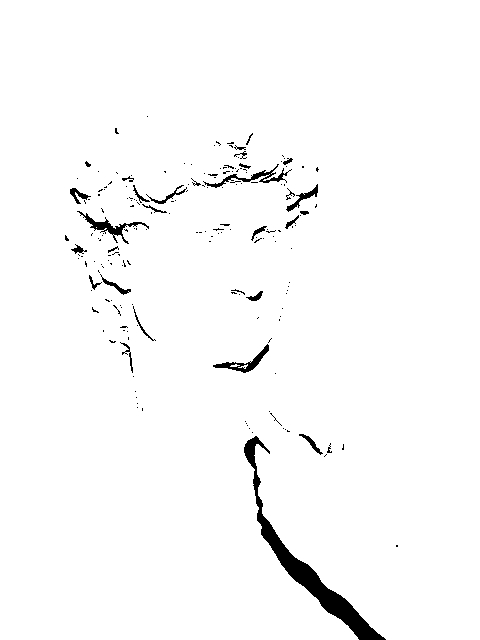
\includegraphics[scale=0.18]{a.jpg}
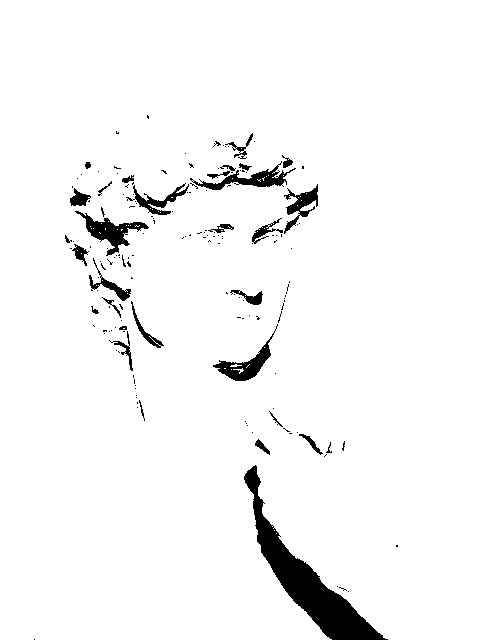
\includegraphics[scale=0.18]{b.jpg}
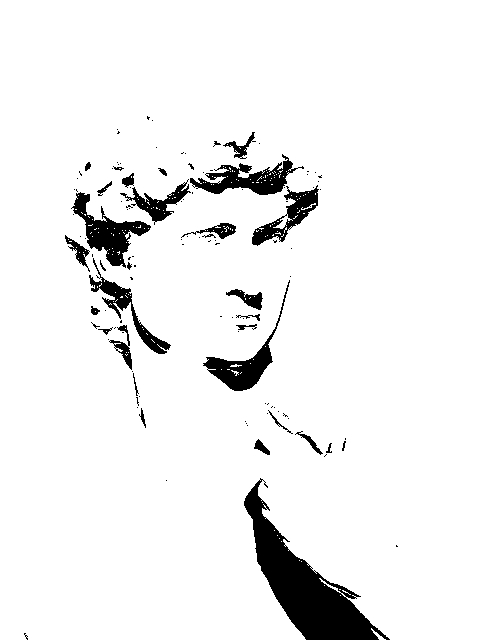
\includegraphics[scale=0.18]{c.jpg}
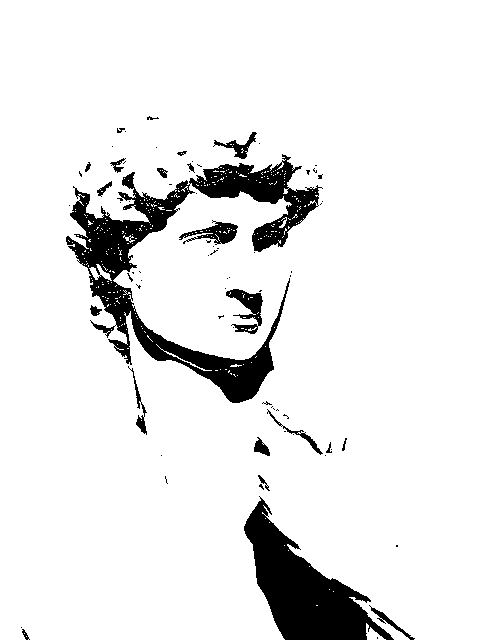
\includegraphics[scale=0.18]{d.jpg}
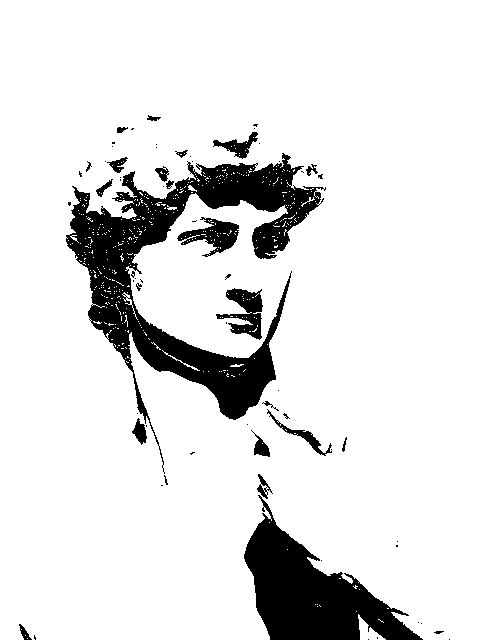
\includegraphics[scale=0.18]{e.jpg}

\section{problem statement}	
We are given a sequence of pictures of a diffusive object with various lighting conditions. \\
We know that in diffusive object, there are 3 basis functions that span all the possible pictures (determined by lighting direction). \\
And we would like to add shadows to this problem. the problem with shadows is that it can not be represented by a low amount of basis functions. \\
So we are seeking a smart interpolation for the representation of the missing parts between the images.

\newpage

\section{Simple interpolation }
Given 2 pictures of logical shadow representation $I_0$ and $I_1$ where
$I_i \in \left\{ 0,1 \right\} ^ {H \times W}$ \\
$I_i$ is the shadow representation of image i. \\
We are seeking a vector mapping $$\Phi _v(t):\mathbb{R}^2\rightarrow\mathbb{R}^2$$
  $$ x\mapsto\Phi _v(t;x)$$
  With the constraints
$$\Phi _v(0) = id$$
$$I_1=I_0\cdot\Phi _v(1)$$
As an initial idea we will define $\Phi _v$ as 
$$\Phi _v = id + t \cdot v$$
This is just an initial model for the vector field and it is going to be changed when we advance with the project.
\\
\\
We define our discrete domain as a graph: $D:=(\nu,\varepsilon,f)$ \\
Where $\nu$ is set of image vertices (pixel corner) \\
$\varepsilon$ as the edges
and $f$ is image faces (pixel center)
\\
Using this definition, assuming there are $n$ vertices and $m$ faces, we define

\begin{center}
Image $I:\nu \rightarrow \mathbb{R} ,\ I \in \mathbb{R}^n $ \\
Vector field velocity $v:f \rightarrow \mathbb{R}^2 ,\ v \in \mathbb{R}^{2m} $
\end{center}

We want to calculate $\phi_v$ by minimizing 
$$ \argmin _v {\|I_1 - I_0 \cdot \Phi _v(1) \|}^2_D =
	\int \limits_D {\|I_1(x) - I_0(x) \cdot \Phi _v(1;x) \|}^2_D dx
$$
\\
This is an ill-posed problem, so we define a regularizing term as follows
$$ \int \limits_D \langle v, \triangle v \rangle da $$
\\
So our minimization problem is
$$ \displaystyle{ \argmin _v \frac{1}{2} \|v\|_{D,\triangle}  + \frac{1}{2 \sigma^2} {\|I_1 - I_0 \cdot \Phi _v(1) \|}^2_D }$$

\newpage
Calculating the regularization term in matrix form:
\begin{eqnarray}
\int \limits_D \langle v, \triangle v \rangle da &=& \\
\sum \limits_{j \in f} A_f(j) \cdot v(j)^T \cdot \triangle v(j) &=& \\
v^T \cdot A_f \cdot \triangle v
\end{eqnarray}
Where $A_f$ is a diagonal matrix of vertices areas. \\

Calculating the data fidelity term in matrix form:
\begin{eqnarray}
\int \limits_D {\|I_1 - I_0 \cdot \Phi _v(1) \|}^2_D \ da \\
\sum \limits_{i \in v} A_v(i) \cdot {\left(I_1(i) - I_0(i) \cdot \Phi _v(1;i) \right)}^2
\end{eqnarray}
Assigning $ \Phi _v(1;i) $ for every i, we get $ \Phi _v(1;i) = id(i) - v(i) $
using bilinear interpolation from faces to vertices \\
Where $ \displaystyle{v(i) = \frac{\sum \limits_{j \in N(i)} v(j)}{\sum \limits_{j \in N(i)} 1}} $  \\
is the mean value of the 1-ring of vertex i.
\begin{eqnarray}
\sum \limits_{i \in v} A_v(i) \cdot {\left[I_1(i) - I_0(i) \cdot (id(i) - v(i)) \right]}^2 = \\
\sum \limits_{i \in v} A_v(i) \cdot 
{\left[
 I_1^2(i) -2 I_0(i) I_1(i) (id(i) - v(i))
 + I_0^2(i)(id(i) - v(i))^2
\right]} = \\
\sum \limits_{i \in v} A_v(i) \cdot
\left\{
[I_0^2(i)] \cdot v^2(i) +
[2I_0(i)I_1(i)-2I_0^2(i)] \cdot v(i) +
[I_1^2(i) -2I_0(i)I_1(i) + I_0^2(i)]
\right\} = \\
A_v \cdot [v^T I_0^ T I_0 v + 2 v^T I_0^T (I_1-I_0) + (I_1-I_0)^2]
\end{eqnarray}
We got a quadratic form $A_v \cdot [v^T K v -2 V^T f + c ]$ where \\
$K = I_0^ T I_0$ is PSD Matrix $(K \geq 0)$ \\
$f =  - I_0^T (I_1-I_0) $ \\
$c = (I_1-I_0)^T (I_1-I_0) $


\newpage

find $v^{opt}$

\begin{eqnarray}
v^{opt} = 
\argmin _v \frac{1}{2}
v^T A_f \triangle v + \frac{1}{2 \sigma^2}
(I_1 - I_0 + v \cdot I_0)^T
A_v
(I_1 - I_0 + v \cdot I_0)
\end{eqnarray}

derivative:
\begin{eqnarray}
\frac{dE}{dv} = 
A_f \triangle v + 
\frac{1}{\sigma^2} I_0^T A_v (I_1 - I_0 + v I_0)
\end{eqnarray}

Steepest Descent:
\begin{eqnarray}
v^{k+1} = v^k - \alpha \frac{dE}{dv}
\end{eqnarray}

\end{document}



